\section{ER-modell}

\subsection{Diagram}

\vspace{1cm}

\makebox[\textwidth][c]{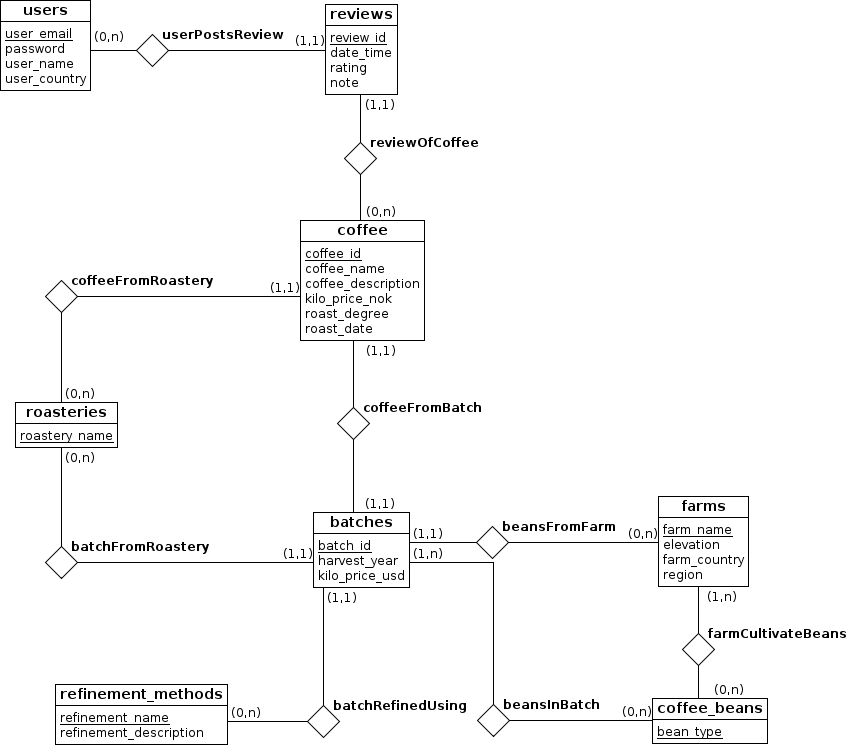
\includegraphics[width=1.2\textwidth]{er-diagram.png}}


\pagebreak

\subsection{Antakelser}

\begin{itemize}
    \item En epost-adresse er knyttet til en-og-bare-en bruker.
    \item Et parti med kaffebønner brukes til en-og-bare-en type kaffe.
    \item Brennerier gir unike navn til egne kaffer (ulike brennerier kan benytte like navn).
    \item Alle foredlingsmetoder har unike navn.
    \item Alle gårder har unike navn.
    \item \textbf{coffee.}\verb|kilo_price_nok| er kiloprisen for kaffen i NOK.
    \item \textbf{batches.}\verb|kilo_price_usd| er i betaling til gård per kilo med bønner i USD.
    \item \textbf{farms.}\verb|elevation| er høyde over havet i meter.
\end{itemize}

\subsection{Kommentarer}

\begin{itemize}
    \item Vi bruker \verb|coffee_id| som primærnøkkel i \class{coffee}-klassen og krever samtidig at alle kombinasjoner av (\verb|coffe_name|, \verb|roastery_name|) må være unike.
    \begin{itemize}
        \item Det betyr at (\verb|coffe_name|, \verb|roastery_name|) kan brukes som sammensatt primærnøkkel.
        \item Isåfall vil \verb|coffee_name| være en delvis nøkkel med identifiserende relasjonsklasse til \class{roasteries}.
        \item I stedet genererer vi surrogatnøkkelen \verb|coffee_id|, fordi det er mer naturlig for administrator av databasen å skille kaffetyper på ett attributt.
        \item Siden \verb|coffee_id| unikt identifiserer entiteter blir \class{coffee} en regulær relasjonsklasse.
    \end{itemize}
    \item Tilsvarende gjelder også nøkkelen \verb|review_id| i \class{reviews}-klassen.
    \begin{itemize}
        \item  (\verb|user_email|, \verb|coffee_id|, \verb|date_time|) kunne alternativt vært brukt som primærnøkkel.
    \end{itemize}
    \item Det kan tenkes at et brenneri ønsker å benytte samme kaffenavn for ulike produksjoner.
    \begin{itemize}
        \item F.eks. om de vil opprettholde merkevaren "Morgenkaffe" over tid.
        \item En slik mini-verden har vanskelig for å tilfredsstille brukerhistorie 1, hvor kaffenavn og brenneri alene skal gi en unik kaffetype.
        \item Dette kunne bl.a. vært løst ved å anta at brukerinput gjelder nyeste produksjon, men vi har i stedet valgt vår restriksjon fordi det gir en mer oversiktlig modell.
    \end{itemize}
\end{itemize}